\chapter{贪心算法}

\index{贪心算法}

\key{贪心算法}通过在每一步
选择当前看起来最优的方案
来构造问题的解。
贪心算法不会撤回已做出的选择，
而是直接构造最终解。
因此，贪心算法通常非常高效。

设计贪心算法的难点在于找到一个
贪心策略，使得该策略总能产生
问题的最优解。
贪心算法中的局部最优选择
也应该是全局最优的。
要论证一个贪心算法的正确性
通常是困难的。

\section{硬币问题}

作为第一个例子，我们考虑这样一个问题：
给定一组硬币，
我们的任务是使用这些硬币
凑出一个金额 $n$。
硬币的面值为
$\texttt{coins}=\{c_1,c_2,\ldots,c_k\}$，
每种硬币可以无限次使用。
最少需要多少枚硬币？

例如，如果硬币是欧元硬币（单位：分）
\[\{1,2,5,10,20,50,100,200\}\]
且 $n=520$，
我们至少需要四枚硬币。
最优解是选择硬币
$200+200+100+20$，其总和为 520。

\subsubsection{贪心算法}

一个简单的贪心算法
总是选择尽可能大的硬币，
直到凑出所需的金额。
这个算法在示例情况下是有效的，
因为我们首先选择两枚 200 分的硬币，
然后选择一枚 100 分的硬币，
最后选择一枚 20 分的硬币。
但这个算法是否总是有效呢？

事实证明，如果硬币是欧元硬币，
贪心算法\emph{总是}有效的，也就是说，
它总是产生一个使用最少硬币数的解。
该算法的正确性可以
通过以下方式证明：

首先，硬币 1、5、10、50 和 100
在最优解中最多出现一次，
因为如果解中包含两枚这样的硬币，
我们可以用一枚硬币替换它们
从而得到更好的解。
例如，如果解中包含硬币 $5+5$，
我们可以用硬币 $10$ 替换它们。

同样地，硬币 2 和 20
在最优解中最多出现两次，
因为我们可以将
硬币 $2+2+2$ 替换为硬币 $5+1$，
将硬币 $20+20+20$ 替换为硬币 $50+10$。
此外，最优解不可能包含
硬币 $2+2+1$ 或 $20+20+10$，
因为我们可以将它们分别替换为硬币 $5$ 和 $50$。

利用这些观察结果，
我们可以对每个硬币 $x$ 证明：
仅使用比 $x$ 小的硬币，
不可能最优地凑出
$x$ 或更大的金额。
例如，如果 $x=100$，使用较小的硬币
能凑出的最大最优和是 $50+20+20+5+2+2=99$。
因此，总是选择最大硬币的贪心算法
产生最优解。

这个例子说明，即使算法本身很简单，
要论证贪心算法的正确性
也可能是困难的。

\subsubsection{一般情况}

在一般情况下，硬币集合可以包含任意硬币，
贪心算法\emph{不一定}能产生
最优解。

我们可以通过给出一个反例
（即算法给出错误答案的情况）
来证明某个贪心算法不正确。
在这个问题中，我们可以很容易地找到一个反例：
如果硬币为 $\{1,3,4\}$ 且目标金额
为 6，贪心算法产生的解为
$4+1+1$，而最优解为 $3+3$。

目前尚不知道一般的硬币问题
是否可以用任何贪心算法来解决\footnote{然而，可以在多项式时间内\emph{检验}
本章中给出的贪心算法对于给定的硬币集合是否有效 \cite{pea05}。}。
但是，正如我们在第 7 章中将看到的，
在某些情况下，
一般问题可以
使用动态规划算法高效求解，
该算法总能给出正确的答案。

\section{调度}

许多调度问题可以用贪心算法来解决。
一个经典问题如下：
给定 $n$ 个事件及其开始时间和结束时间，
找到一个能包含尽可能多事件的安排方案。
不能部分地选择一个事件。
例如，考虑以下事件：
\begin{center}
\begin{tabular}{lll}
事件 & 开始时间 & 结束时间 \\
\hline
$A$ & 1 & 3 \\
$B$ & 2 & 5 \\
$C$ & 3 & 9 \\
$D$ & 6 & 8 \\
\end{tabular}
\end{center}
在这种情况下，最多可以选择两个事件。
例如，我们可以选择事件 $B$ 和 $D$，
如下所示：
\begin{center}
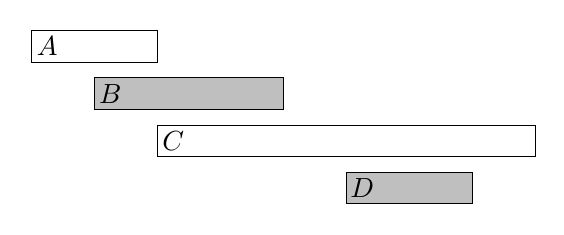
\begin{tikzpicture}[scale=.4]
  \begin{scope}
    \draw (2, 0) rectangle (6, -1);
    \draw[fill=lightgray] (4, -1.5) rectangle (10, -2.5);
    \draw (6, -3) rectangle (18, -4);
    \draw[fill=lightgray] (12, -4.5) rectangle (16, -5.5);
    \node at (2.5,-0.5) {$A$};
    \node at (4.5,-2) {$B$};
    \node at (6.5,-3.5) {$C$};
    \node at (12.5,-5) {$D$};
  \end{scope}
\end{tikzpicture}
\end{center}

对于这个问题，可以想到多种贪心算法，
但哪些算法在所有情况下都有效呢？

\subsubsection*{算法 1}

第一个想法是尽可能选择\emph{短的}
事件。
在示例情况下，这个算法
选择以下事件：
\begin{center}
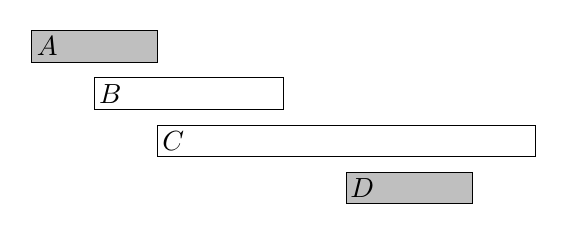
\begin{tikzpicture}[scale=.4]
  \begin{scope}
    \draw[fill=lightgray] (2, 0) rectangle (6, -1);
    \draw (4, -1.5) rectangle (10, -2.5);
    \draw (6, -3) rectangle (18, -4);
    \draw[fill=lightgray] (12, -4.5) rectangle (16, -5.5);
    \node at (2.5,-0.5) {$A$};
    \node at (4.5,-2) {$B$};
    \node at (6.5,-3.5) {$C$};
    \node at (12.5,-5) {$D$};
  \end{scope}
\end{tikzpicture}
\end{center}

然而，选择短事件并不总是一个
正确的策略。例如，算法在以下情况中失败：
\begin{center}
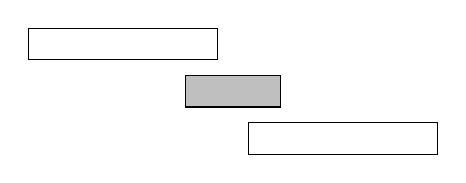
\begin{tikzpicture}[scale=.4]
  \begin{scope}
    \draw (1, 0) rectangle (7, -1);
    \draw[fill=lightgray] (6, -1.5) rectangle (9, -2.5);
    \draw (8, -3) rectangle (14, -4);
  \end{scope}
\end{tikzpicture}
\end{center}
如果我们选择了短事件，就只能选择一个事件。
然而，本来可以选择两个长事件的。

\subsubsection*{算法 2}

另一个想法是总是选择下一个
\emph{开始}尽可能\emph{早}的可用事件。
这个算法选择以下事件：
\begin{center}
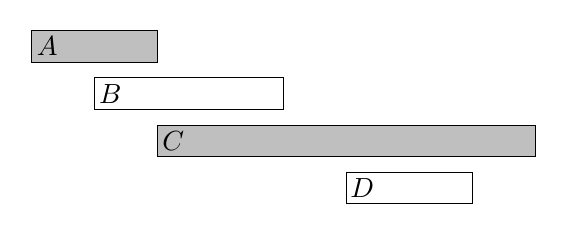
\begin{tikzpicture}[scale=.4]
  \begin{scope}
    \draw[fill=lightgray] (2, 0) rectangle (6, -1);
    \draw (4, -1.5) rectangle (10, -2.5);
    \draw[fill=lightgray] (6, -3) rectangle (18, -4);
    \draw (12, -4.5) rectangle (16, -5.5);
    \node at (2.5,-0.5) {$A$};
    \node at (4.5,-2) {$B$};
    \node at (6.5,-3.5) {$C$};
    \node at (12.5,-5) {$D$};
  \end{scope}
\end{tikzpicture}
\end{center}

然而，我们也可以为这个算法
找到一个反例。
例如，在以下情况中，
算法只选择了一个事件：
\begin{center}
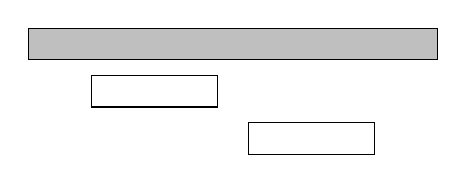
\begin{tikzpicture}[scale=.4]
  \begin{scope}
    \draw[fill=lightgray] (1, 0) rectangle (14, -1);
    \draw (3, -1.5) rectangle (7, -2.5);
    \draw (8, -3) rectangle (12, -4);
  \end{scope}
\end{tikzpicture}
\end{center}
如果我们选择了第一个事件，就无法
再选择任何其他事件。
然而，本来可以选择
另外两个事件的。

\subsubsection*{算法 3}

第三个想法是总是选择下一个
\emph{结束}尽可能\emph{早}的可用事件。
这个算法选择以下事件：
\begin{center}
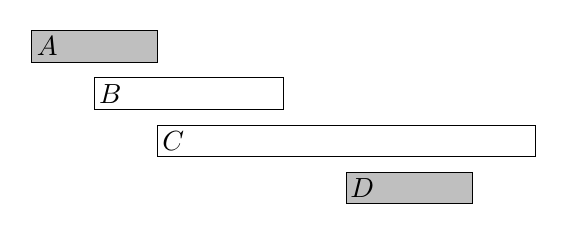
\begin{tikzpicture}[scale=.4]
  \begin{scope}
    \draw[fill=lightgray] (2, 0) rectangle (6, -1);
    \draw (4, -1.5) rectangle (10, -2.5);
    \draw (6, -3) rectangle (18, -4);
    \draw[fill=lightgray] (12, -4.5) rectangle (16, -5.5);
    \node at (2.5,-0.5) {$A$};
    \node at (4.5,-2) {$B$};
    \node at (6.5,-3.5) {$C$};
    \node at (12.5,-5) {$D$};
  \end{scope}
\end{tikzpicture}
\end{center}

事实证明，这个算法
\emph{总是}能产生最优解。
原因是：首先选择一个结束时间尽可能早的事件
总是最优选择。
之后，使用相同的策略选择下一个事件
也是最优选择，以此类推，
直到我们无法再选择更多事件为止。

论证该算法正确性的一种方式是
考虑：如果我们首先选择一个
比最早结束事件结束得更晚的事件，
会发生什么。
此时，我们在选择下一个事件时
最多只能有相同数量的可选方案。
因此，选择一个结束更晚的事件
永远不会产生更好的解，
所以贪心算法是正确的。

\section{任务与截止时间}

现在我们来考虑这样一个问题：
给定 $n$ 个任务，每个任务有其持续时间和截止时间，
我们的任务是选择一个执行任务的顺序。
对于每个任务，我们获得 $d-x$ 分，
其中 $d$ 是任务的截止时间，
$x$ 是我们完成任务的时刻。
我们能获得的最高总分是多少？

例如，假设任务如下：
\begin{center}
\begin{tabular}{lll}
任务 & 持续时间 & 截止时间 \\
\hline
$A$ & 4 & 2 \\
$B$ & 3 & 5 \\
$C$ & 2 & 7 \\
$D$ & 4 & 5 \\
\end{tabular}
\end{center}
在这种情况下，任务的一个最优安排方案
如下：
\begin{center}
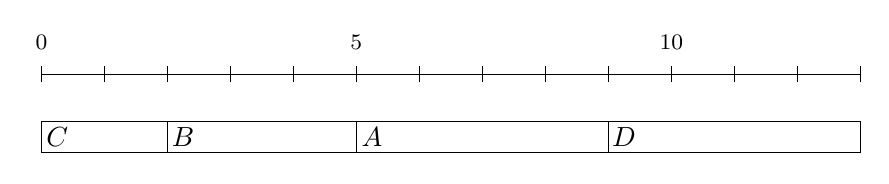
\begin{tikzpicture}[scale=.4]
  \begin{scope}
    \draw (0, 0) rectangle (4, -1);
    \draw (4, 0) rectangle (10, -1);
    \draw (10, 0) rectangle (18, -1);
    \draw (18, 0) rectangle (26, -1);
    \node at (0.5,-0.5) {$C$};
    \node at (4.5,-0.5) {$B$};
    \node at (10.5,-0.5) {$A$};
    \node at (18.5,-0.5) {$D$};

    \draw (0,1.5) -- (26,1.5);
    \foreach \i in {0,2,...,26}
    {
        \draw (\i,1.25) -- (\i,1.75);
    }
    \footnotesize
    \node at (0,2.5) {0};
    \node at (10,2.5) {5};
    \node at (20,2.5) {10};

  \end{scope}
\end{tikzpicture}
\end{center}
在这个方案中，$C$ 获得 5 分，
$B$ 获得 0 分，$A$ 获得 $-7$ 分，
$D$ 获得 $-8$ 分，
所以总分为 $-10$。

令人惊讶的是，这个问题的最优解
完全不依赖于截止时间，
正确的贪心策略仅仅是
将任务\emph{按持续时间排序}，
然后按递增顺序执行。
原因是，如果我们连续执行两个任务，
而第一个任务比第二个任务耗时更长，
那么交换这两个任务可以得到更好的解。
例如，考虑以下安排：
\begin{center}
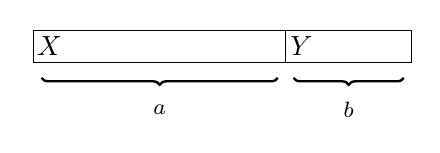
\begin{tikzpicture}[scale=.4]
  \begin{scope}
    \draw (0, 0) rectangle (8, -1);
    \draw (8, 0) rectangle (12, -1);
    \node at (0.5,-0.5) {$X$};
    \node at (8.5,-0.5) {$Y$};

\draw [decoration={brace}, decorate, line width=0.3mm] (7.75,-1.5) -- (0.25,-1.5);
\draw [decoration={brace}, decorate, line width=0.3mm] (11.75,-1.5) -- (8.25,-1.5);

\footnotesize
\node at (4,-2.5) {$a$};
\node at (10,-2.5) {$b$};

  \end{scope}
\end{tikzpicture}
\end{center}
这里 $a>b$，所以我们应该交换任务：
\begin{center}
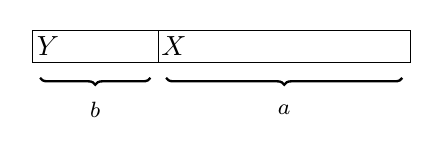
\begin{tikzpicture}[scale=.4]
  \begin{scope}
    \draw (0, 0) rectangle (4, -1);
    \draw (4, 0) rectangle (12, -1);
    \node at (0.5,-0.5) {$Y$};
    \node at (4.5,-0.5) {$X$};

\draw [decoration={brace}, decorate, line width=0.3mm] (3.75,-1.5) -- (0.25,-1.5);
\draw [decoration={brace}, decorate, line width=0.3mm] (11.75,-1.5) -- (4.25,-1.5);

\footnotesize
\node at (2,-2.5) {$b$};
\node at (8,-2.5) {$a$};

  \end{scope}
\end{tikzpicture}
\end{center}
现在 $X$ 少得 $b$ 分，$Y$ 多得 $a$ 分，
所以总分增加了 $a-b > 0$。
在最优解中，对于任意两个连续的任务，
必须保证较短的任务在
较长的任务之前。
因此，任务必须按其持续时间
排序后执行。

\section{最小化和}

接下来我们考虑这样一个问题：
给定 $n$ 个数 $a_1,a_2,\ldots,a_n$，
我们的任务是找到一个值 $x$，
使得以下和最小：
\[|a_1-x|^c+|a_2-x|^c+\cdots+|a_n-x|^c.\]
我们重点关注 $c=1$ 和 $c=2$ 的情况。

\subsubsection{情况 $c=1$}

在这种情况下，我们应该最小化和
\[|a_1-x|+|a_2-x|+\cdots+|a_n-x|.\]
例如，如果这些数是 $[1,2,9,2,6]$，
最好的解是选择 $x=2$，
产生的和为
\[
|1-2|+|2-2|+|9-2|+|2-2|+|6-2|=12.
\]
在一般情况下，$x$ 的最佳选择
是这些数的\textit{中位数}，
即排序后位于中间的数。
例如，列表 $[1,2,9,2,6]$
排序后变为 $[1,2,2,6,9]$，
所以中位数是 2。

中位数是最优选择，
因为如果 $x$ 小于中位数，
增大 $x$ 会使和变小；
如果 $x$ 大于中位数，
减小 $x$ 会使和变小。
因此，最优解是令 $x$
为中位数。
如果 $n$ 是偶数且有两个中位数，
则两个中位数以及它们之间的所有值
都是最优选择。

\subsubsection{情况 $c=2$}

在这种情况下，我们应该最小化和
\[(a_1-x)^2+(a_2-x)^2+\cdots+(a_n-x)^2.\]
例如，如果这些数是 $[1,2,9,2,6]$，
最好的解是选择 $x=4$，
产生的和为
\[
(1-4)^2+(2-4)^2+(9-4)^2+(2-4)^2+(6-4)^2=46.
\]
在一般情况下，$x$ 的最佳选择
是这些数的\emph{平均值}。
在示例中，平均值为 $(1+2+9+2+6)/5=4$。
这个结果可以通过将和表示如下来推导：
\[
nx^2 - 2x(a_1+a_2+\cdots+a_n) + (a_1^2+a_2^2+\cdots+a_n^2)
\]
最后一部分不依赖于 $x$，
所以我们可以忽略它。
剩余部分构成函数
$nx^2-2xs$，其中 $s=a_1+a_2+\cdots+a_n$。
这是一个开口向上的抛物线，
其根为 $x=0$ 和 $x=2s/n$，
最小值为两根的平均值
$x=s/n$，即
数 $a_1,a_2,\ldots,a_n$ 的平均值。

\section{数据压缩}

\index{数据压缩}
\index{二进制码}
\index{码字}

\key{二进制码}为字符串中的每个字符
分配一个由比特组成的\key{码字}。
我们可以使用二进制码\emph{压缩}字符串，
方法是将每个字符替换为
对应的码字。
例如，以下二进制码
为字符 \texttt{A}–\texttt{D} 分配码字：
\begin{center}
\begin{tabular}{rr}
字符 & 码字 \\
\hline
\texttt{A} & 00 \\
\texttt{B} & 01 \\
\texttt{C} & 10 \\
\texttt{D} & 11 \\
\end{tabular}
\end{center}
这是一种\key{定长}码，
意味着每个码字的长度相同。
例如，我们可以将字符串
\texttt{AABACDACA} 压缩如下：
\[00\,00\,01\,00\,10\,11\,00\,10\,00\]
使用这种编码，压缩后的
字符串长度为 18 比特。
然而，如果我们使用\key{变长}码
（其中码字可以有不同的长度），
就可以更好地压缩字符串。
这样我们可以为经常出现的字符
分配较短的码字，
为很少出现的字符
分配较长的码字。
事实证明，上述字符串的一个\key{最优}码
如下：
\begin{center}
\begin{tabular}{rr}
字符 & 码字 \\
\hline
\texttt{A} & 0 \\
\texttt{B} & 110 \\
\texttt{C} & 10 \\
\texttt{D} & 111 \\
\end{tabular}
\end{center}
最优码产生尽可能短的
压缩字符串。
在这种情况下，使用最优码压缩后的
字符串为
\[0\,0\,110\,0\,10\,111\,0\,10\,0,\]
所以只需要 15 比特，而不是 18 比特。
因此，得益于更好的编码，
压缩字符串中节省了 3 比特。

我们要求没有任何码字
是另一个码字的前缀。
例如，不允许一个编码
同时包含码字 10
和 1011。
原因是我们希望能够从压缩字符串
还原出原始字符串。
如果一个码字可以是另一个码字的前缀，
这就不是总能做到的。
例如，以下编码是\emph{无效}的：
\begin{center}
\begin{tabular}{rr}
字符 & 码字 \\
\hline
\texttt{A} & 10 \\
\texttt{B} & 11 \\
\texttt{C} & 1011 \\
\texttt{D} & 111 \\
\end{tabular}
\end{center}
使用这种编码，我们无法确定
压缩字符串 1011 对应的是
字符串 \texttt{AB} 还是字符串 \texttt{C}。

\index{哈夫曼编码}

\subsubsection{哈夫曼编码}

\key{哈夫曼编码}\footnote{D. A. Huffman 在解答一门大学课程的作业时发现了这种方法，
并于 1952 年发表了该算法 \cite{huf52}。}是一种贪心算法，
用于构造压缩给定字符串的
最优编码。
该算法基于字符串中各字符的频率
构建一棵二叉树，
每个字符的码字可以通过
从根节点到对应节点的路径来读取。
向左走对应比特 0，
向右走对应比特 1。

初始时，字符串中的每个字符由一个
节点表示，其权重为该字符
在字符串中出现的次数。
然后在每一步中，选择权重最小的两个节点
进行合并，创建一个新节点，
其权重为原始两个节点权重之和。
这个过程持续进行，直到所有节点都被合并。

接下来我们将看到哈夫曼编码如何
为字符串 \texttt{AABACDACA}
创建最优编码。
初始时，有四个节点分别对应
字符串中的字符：

\begin{center}
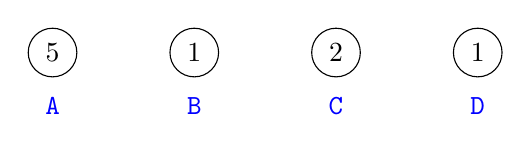
\begin{tikzpicture}[scale=0.9]
\node[draw, circle] (1) at (0,0) {$5$};
\node[draw, circle] (2) at (2,0) {$1$};
\node[draw, circle] (3) at (4,0) {$2$};
\node[draw, circle] (4) at (6,0) {$1$};

\node[color=blue] at (0,-0.75) {\texttt{A}};
\node[color=blue] at (2,-0.75) {\texttt{B}};
\node[color=blue] at (4,-0.75) {\texttt{C}};
\node[color=blue] at (6,-0.75) {\texttt{D}};

%\path[draw,thick,-] (4) -- (5);
\end{tikzpicture}
\end{center}
表示字符 \texttt{A} 的节点
权重为 5，因为字符 \texttt{A}
在字符串中出现了 5 次。
其他权重以相同的方式
计算得到。

第一步是合并对应字符 \texttt{B} 和 \texttt{D}
的节点，两者的权重都是 1。
结果如下：
\begin{center}
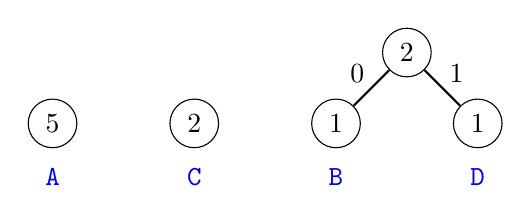
\begin{tikzpicture}[scale=0.9]
\node[draw, circle] (1) at (0,0) {$5$};
\node[draw, circle] (3) at (2,0) {$2$};
\node[draw, circle] (2) at (4,0) {$1$};
\node[draw, circle] (4) at (6,0) {$1$};
\node[draw, circle] (5) at (5,1) {$2$};

\node[color=blue] at (0,-0.75) {\texttt{A}};
\node[color=blue] at (2,-0.75) {\texttt{C}};
\node[color=blue] at (4,-0.75) {\texttt{B}};
\node[color=blue] at (6,-0.75) {\texttt{D}};

\node at (4.3,0.7) {0};
\node at (5.7,0.7) {1};

\path[draw,thick,-] (2) -- (5);
\path[draw,thick,-] (4) -- (5);
\end{tikzpicture}
\end{center}
之后，权重为 2 的节点被合并：
\begin{center}
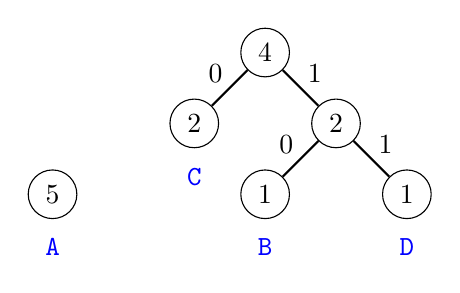
\begin{tikzpicture}[scale=0.9]
\node[draw, circle] (1) at (1,0) {$5$};
\node[draw, circle] (3) at (3,1) {$2$};
\node[draw, circle] (2) at (4,0) {$1$};
\node[draw, circle] (4) at (6,0) {$1$};
\node[draw, circle] (5) at (5,1) {$2$};
\node[draw, circle] (6) at (4,2) {$4$};

\node[color=blue] at (1,-0.75) {\texttt{A}};
\node[color=blue] at (3,1-0.75) {\texttt{C}};
\node[color=blue] at (4,-0.75) {\texttt{B}};
\node[color=blue] at (6,-0.75) {\texttt{D}};

\node at (4.3,0.7) {0};
\node at (5.7,0.7) {1};
\node at (3.3,1.7) {0};
\node at (4.7,1.7) {1};

\path[draw,thick,-] (2) -- (5);
\path[draw,thick,-] (4) -- (5);
\path[draw,thick,-] (3) -- (6);
\path[draw,thick,-] (5) -- (6);
\end{tikzpicture}
\end{center}
最后，合并剩下的两个节点：
\begin{center}
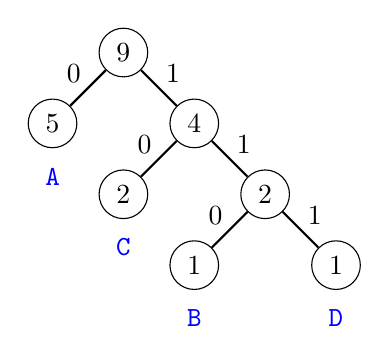
\begin{tikzpicture}[scale=0.9]
\node[draw, circle] (1) at (2,2) {$5$};
\node[draw, circle] (3) at (3,1) {$2$};
\node[draw, circle] (2) at (4,0) {$1$};
\node[draw, circle] (4) at (6,0) {$1$};
\node[draw, circle] (5) at (5,1) {$2$};
\node[draw, circle] (6) at (4,2) {$4$};
\node[draw, circle] (7) at (3,3) {$9$};

\node[color=blue] at (2,2-0.75) {\texttt{A}};
\node[color=blue] at (3,1-0.75) {\texttt{C}};
\node[color=blue] at (4,-0.75) {\texttt{B}};
\node[color=blue] at (6,-0.75) {\texttt{D}};

\node at (4.3,0.7) {0};
\node at (5.7,0.7) {1};
\node at (3.3,1.7) {0};
\node at (4.7,1.7) {1};
\node at (2.3,2.7) {0};
\node at (3.7,2.7) {1};

\path[draw,thick,-] (2) -- (5);
\path[draw,thick,-] (4) -- (5);
\path[draw,thick,-] (3) -- (6);
\path[draw,thick,-] (5) -- (6);
\path[draw,thick,-] (1) -- (7);
\path[draw,thick,-] (6) -- (7);
\end{tikzpicture}
\end{center}

现在所有节点都在树中了，编码已完成。
从树中可以读取以下码字：
\begin{center}
\begin{tabular}{rr}
字符 & 码字 \\
\hline
\texttt{A} & 0 \\
\texttt{B} & 110 \\
\texttt{C} & 10 \\
\texttt{D} & 111 \\
\end{tabular}
\end{center}
